\section*{Opción A:}
\begin{mybox}
    \paragraph{A.1-}En una obra, para transportar la tierra extraída para la construcción de los cimientos de un edificio, se usan tres
    tipos de camiones diferentes: $A$, $B$ y $C$. Los camiones de tipo $A$ tienen una capacidad de 14 toneladas, los de
    tipo $B$, de 24 toneladas y los de tipo $C$, de 28 toneladas. Habría que traer un camión más de tipo $A$ para igualar
    al número de camiones restantes. El $10\%$ de la capacidad de todos los camiones tipo $B$ supone un séptimo de la
    de los de mayor tonelaje. Hoy, realizando un único viaje cada camión a máxima capacidad, se han extraído de la
    obra 302 toneladas de tierra. ¿Cuánta tierra ha sido transportada hoy por los camiones de cada tipo? 
\end{mybox}

\paragraph{Solución:} 
En primer lugar, llamaremos al número de camiones de cada tipo $A,B,C$, respectivamente; y la capacidad total de esos camiones será la capacidad de un camión individual por el número de camiones de cada tipo. En forma de tabla, esto es:
\begin{table}[!h]
    \centering
    \begin{tabular}{c|c|c|c}
         $\#$ Camiones& $A$&$B$&$C$  \\ \hline
         Capacidades& $14A$&$24B$&$28C$ 
    \end{tabular}
    \label{tab:my_label}
\end{table}\\
Como la capacidad total de todos los camiones (la suma de la segunda fila) tiene que ser 302 toneladas, obtenemos una primera ecuación.
\begin{equation}
    \boxed{14A+24B+28C=302}
\end{equation}
Por otro lado, para que el número de camiones de tipo $A$ sea igual al número de camiones de los tipos restantes, necesitamos añadir un camión de tipo $A$ a los que ya tenemos. Esto es nuestra segunda ecuación.
\begin{equation}
    \boxed{A+1=B+C}
\end{equation}
Por último, sabemos que el $10\%$ de la capacidad de $B$ ($10\%$ de $24B$) supone un séptimo de la capacidad de los camiones de \emph{mayor} tonelaje, es decir, la capacidad de $C$ ($28C$). Con esto obtenemos nuestra última ecuación.
\begin{equation}
    10\% \text{ de } 24B=\frac{1}{7} \text{ de } 28C\implies \boxed{2.4B=4C}
\end{equation}
Y tenemos finalmente un sistema de ecuaciones lineales con tres incógnitas:
$$
\left \{ \begin{array}{ccccc}
     14A&+\phantom{.}24B  &+28C&=&302  \\
     \phantom{14}A  &-\phantom{24}B    &-\phantom{28}C  &=&-1\\
        & \phantom{-}2.4B &-\phantom{8}4C &=&0
\end{array} \right .
$$
Este sistema puede resolverse de muchas maneras. En este caso, empleo la eliminación gaussiana. En forma matricial:
$$
\left [ \begin{array}{ccc|c}
    14 &24&28&302  \\
    1 & -1&-1&-1   \\
    0& 2.4& -4 &0
\end{array} \right ] \xlongrightarrow{F_2'=14 F_2 -F_1} \left [ \begin{array}{ccc|c}
    14 &24&28&302  \\
    0 & -38&-42&-316   \\
    0& 2.4& -4 &0
\end{array} \right ]\xlongrightarrow{F_3'=(38/2.4) \ F_3 +F_2}
$$
\begin{align*}
\left [ \begin{array}{ccc|c}
    14 &24&28&302  \\
    0 & -38&-42&-316   \\
    0& 0& -316/3 &-316
\end{array} \right ] \longrightarrow \left \{ \begin{array}{c}
     -(316/3) \ C=-316  \\
     \implies C=3
\end{array} \right . &\longrightarrow \left \{ \begin{array}{c}
     -38B-42C=-316  \\
     \implies B=5
\end{array} \right .\\ &\longrightarrow \left \{ \begin{array}{c}
     14A+24B+28C=302  \\
     \implies A=7 
\end{array} \right .
\end{align*}
Como nos preguntan cuánta tierra ha sido transportada por cada tipo de camión, el resultado final será: $A: 14\times 7=98$ t, $B: 24\times 5=120$ t y $C: 28\times 3=84$ t.\\

\noindent\rule{\textwidth}{0.5pt}
\begin{mybox}
    \paragraph{A.2-} Dada la función $f(x)=\sqrt[3]{(x^2-1)^2}$, se pide:
    \begin{enumerate}
        \item[(a)] Estudiar si es par o impar.
        \item[(b)] Estudiar su derivabilidad en el punto $x=1$.
        \item[(c)] Estudiar sus extremos relativos y absolutos.
    \end{enumerate}
\end{mybox}
\paragraph{Solución:} $f(x)=\sqrt[3]{(x^2-1)^2}=(x^2-1)^{2/3} \ \ge0$:
\begin{enumerate}
    \item[(a)] Si una función es \emph{par}: $f(-x)=f(x)$. Si una función es \emph{impar}: $f(-x)=-f(x)$.\\
    
    $ f(-x)=\sqrt[3]{((-x)^2-1)^2}=\sqrt[3]{(x^2-1)^2}=f(x)\implies $ La función es \textbf{par.}
    \item[(b)] Para que una función sea derivable en un punto, debe cumplir primero que sea continua en ese punto. Como la función $f(x)$ no tiene problemas de dominio ($D(f)=\mathbb{R}$), es continua en toda la recta real, y por tanto en $x=1$. La condición de derivabilidad es que el límite en $x=1$ de la derivada exista, es decir, $f'(1^+)=f'(1^-)$
    \begin{equation*}
        \begin{split}
            f'(x)&=\frac{2}{3}(x^2-1)^{-1/3}\cdot 2x=\frac{4}{3}\frac{x}{\sqrt[3]{x^2-1}}\\
            &\rightarrow f'(1^+)=\lim_{x\to 1^+} \frac{4}{3}\frac{x}{\sqrt[3]{x^2-1}}=\frac{4}{3}\cdot \frac{1}{0^+}=+\infty\\
            &\rightarrow f'(1^-)=\lim_{x\to 1^-} \frac{4}{3}\frac{x}{\sqrt[3]{x^2-1}}=\frac{4}{3}\cdot \frac{1}{0^-}=-\infty\\
            &\implies \nexists f'(1^\pm) \implies \text{ La función \textbf{no es derivable} en }x=1.
        \end{split}
    \end{equation*}

    \item[(c)] Los extremos \emph{relativos} se estudian igualando la derivada de $f(x)$ a cero y estudiando el crecimiento y decrecimiento de la función.
    \begin{gather*}
        f'(x)=\frac{4}{3}\frac{x}{\sqrt[3]{x^2-1}}\equiv 0\implies \boxed{x=0} \text{ \small  (posible extremo relativo)}.
    \end{gather*}
    Otros puntos a considerar en el crecimiento y decrecimiento de la función son los puntos conflictivos de la derivada, que son $x=\pm 1$ ya que la función no es derivable en esos puntos pero $f(x)$ es continua.
    \begin{table}[!h]
        \centering
        \begin{tabular}{c|c|c|c|c}
           Intervalos  &$(-\infty ,-1)$ & $(-1,0)$     & $(0,1)$     & $(1,+\infty )$  \\ \hline
           $f'(x)$     & $<0$           & $>0$        & $<0$        & $>0$  \\ \hline 
           $f(x)$      &$\searrow $     & $\nearrow $ & $\searrow $ & $\nearrow $ \\
        \end{tabular}
        \label{tab:my_label2}
    \end{table}\\
    En $x=0$, la función alcanza un \textbf{máximo relativo}, cuyo valor es $f(0)=1$. Como la función crece hasta hacerse infinita en $x\to \pm \infty $, \textbf{no hay máximos absolutos}. Con respecto a los mínimos, como la función $f(x) \ge 0 \ \forall x \in \mathbb{R}$, en $x=\pm 1$ la función tiene \textbf{mínimos absolutos} ($f(\pm 1)=0$), y \textbf{no hay mínimos relativos}. 
    \newpage
    Estos resultados que hemos obtenido pueden verse bien en la siguiente gráfica.
    \begin{figure}[!h]
        \centering
        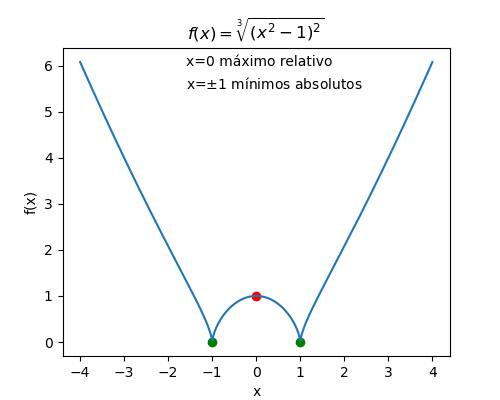
\includegraphics[scale=.7]{evau_2023.png}
        \caption*{$f(x)$ en $[-4,4]$.}
        \label{fig:enter-label}
    \end{figure}
    Como se puede comprobar, la función presenta simetría par. En $x=\pm 1$ la función no es derivable ya que tenemos \emph{picos} (derivadas $\to \pm \infty$) en esos puntos; y presenta un máximo relativo en $x=0$ y mínimos absolutos en $x=\pm 1$.
\end{enumerate}
    
\noindent\rule{\textwidth}{0.5pt}
\begin{mybox}
    \paragraph{A.3-} Sean los puntos $A(1,-2,3)$, $B(0,2,-1)$ y $C(2,1,0)$. Se pide:
    \begin{enumerate}
        \item[(a)] Comprobar que forman un triángulo $T$ y hallar una ecuación del plano que los contiene.
        \item[(b)] Calcular el corte de la recta que pasa por los puntos $A$ y $B$ con el plano $z = 1$.
        \item[(c)] Determinar el perímetro del triángulo $T$. 
    \end{enumerate}
\end{mybox}
\paragraph{Solución:}
\begin{enumerate}
    \item[(a)] Un triángulo está formado por tres lados y tres vértices \emph{que no son colineales}, es decir, que los puntos no están alineados. La manera de comprobar que los puntos $A,B$ y $C$ forman un triángulo es, entonces, comprobar que los puntos no son colineales. Si tres puntos $A,B,C$ \emph{son} colineales, entonces los vectores que forman, $\vec{AB}, \Vec{BC}, \Vec{AC}$ deben ser \emph{linealmente dependientes}. Esto es:
    $$
    \Vec{AB}=\lambda \Vec{AC} 
    $$
    Los vectores $\Vec{AB}$, $\Vec{AC}$ y $\Vec{BC}$ se calculan de la siguiente manera: $\Vec{AB} = B-A=(0,2,-1)-(1,-2,3) = (-1,4,-4)$, $\Vec{AC} = C-A = (2,1,0)-(1,-2,3) = (1,3,-3)$, $\Vec{BC}=C-B=(2,1,0)-(0,2,-1) = (2,-1,1)$. Entonces:
    $$
    \Vec{AB}=(-1,4,-4)=\lambda \Vec{AC}=\lambda (1,3,-3) \implies \begin{cases}
         -1=\lambda \cdot 1    \implies \lambda =-1\\
          4=\lambda \cdot 3    \implies \lambda =4/3\\ 
         -4=\lambda \cdot (-3) \implies \lambda =4/3
    \end{cases}
    $$
    Como no hay un valor de $\lambda$ único, los vectores son linealmente independientes, por lo que los puntos $A,B,C$ \textbf{forman un triángulo}. \\

    Por otro lado, la ecuación del plano que pasa por los tres puntos o, lo que es lo mismo, pasa por el punto $A(a_1,a_2,a_3)$ y tiene como vectores $\Vec{AB}$ y $\Vec{AC}$ es:
    $$
    \pi \equiv \left | \begin{array}{ccc}
        AB_1 & AC_1 & x-a_1  \\
        AB_2 & AC_2 & y-a_2  \\
        AB_3 & AC_2 & z-a_3
    \end{array} \right | =0= \left | \begin{array}{ccc}
        -1 &  1 & x-1  \\
         4 &  3 & y+2  \\
        -4 & -3 & z-3
    \end{array} \right |
    $$
    Calculando el determinante y simplificando, obtenemos que la ecuación del plano $\boxed{\pi \equiv z+y=1}$

    \item[(b)] La recta que pasa por $A$ y $B$ es la recta que pasa por $A$ y tiene un vector $\Vec{AB}=(-1,4,-4)$, que en ecuaciones parametricas es:
    $$
    r\equiv \begin{cases}
        x=1-\lambda \\
        y=-2+4\lambda \\
        z=3-4\lambda 
    \end{cases} \ , \ \lambda \in \mathbb{R}
    $$
    El corte de la recta con este plano es la intersección $r \cap (z=1)\equiv P$.
    $$
    r\cap (z=1) : z=1=3-4\lambda \iff \boxed{\lambda =1/2} \rightarrow \begin{cases}
        x=1-1/2=1/2\\
        y=-2+2=0\\
        z=1
    \end{cases}\implies \boxed{P(1/2,0,1)}
    $$

    \item[(c)] El perímetro del triángulo $T$ se calcula como la suma de los tres lados, es decir:
    \begin{equation*}
        \begin{split}
            p=|\Vec{AB}|+|\Vec{AC}|+|\Vec{BC}|&=\sqrt{1^1+4^2+4^2}+\sqrt{1+3^2+3^2}+\sqrt{2^2+1^2+1^2}\\
                                              &=\sqrt{33}+\sqrt{19}+\sqrt{6} =\boxed{12.55 \text{ u}} 
        \end{split}
    \end{equation*}
\end{enumerate}

\noindent\rule{\textwidth}{0.5pt}
\begin{mybox}
    \paragraph{A.4-} Se tiene un suceso $A$ de probabilidad $P(A) = 0.3$:
    \begin{enumerate}
        \item[(a)] Un suceso $B$ de probabilidad $P(B) = 0.5$ es independiente de $A$. Calcule $P(A \cup B)$. 
        \item[(b)] Otro suceso $C$ cumple $P(C | A) = 0.5$. Determine $P(A \cap \bar{C})$. 
        \item[(c)] Si se tiene un suceso $D$ tal que $P(\Bar{A} | D) = 0.2$ y $P(D | A) = 0.5$, calcule $P(D)$. 
    \end{enumerate}
\end{mybox}
\paragraph{Solución:}
\begin{enumerate}
    \item[(a)] Al ser el suceso $B$ independiente de $A$, entonces $P(A\cap B)=P(A)\cdot P(B)=0.3 \cdot 0.5=0.15$. \\ La probabilidad $P(A\cup B)=P(A)+P(B)-P(A\cap B)=0.3+0.5-0.15=\boxed{0.65}$ 
    \item[(b)] La probabilidad que buscamos está representada en rojo en la siguiente imagen:
    
    \begin{minipage}{.64\textwidth}
    \begin{equation*}
        \begin{split}
            P(A\cap \Bar{C})&=P(A)-P(A\cap C) \\
            P(C|A)&=0.5=\frac{P(A\cap C)}{P(A)}\implies P(A\cap C)=0.15\\
            P(A\cap \Bar{C})&=0.3-0.15=\boxed{0.15}
        \end{split}
    \end{equation*}
    \end{minipage}
    \begin{minipage}{.64\textwidth}
        \setlength{\parindent}{1em}
        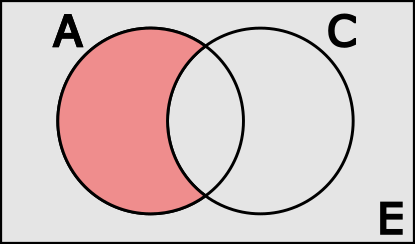
\includegraphics[scale=.4]{g6449.png}
    \end{minipage}

    \item[(c)] $P(\Bar{A}|D)=0.2=\dfrac{P(\Bar{A}\cap D)}{P(D)}=\dfrac{P(D)-P(D\cap A)}{P(D)}$ \small (mismo razonamiento que ap. b) \normalsize\\
    Además:\\
    $
    P(D|A)=0.5=\dfrac{P(D\cap A)}{P(A)}=\dfrac{P(D\cap A)}{0.3}\implies P(D\cap A)=0.15.
    $ Por tanto, obtenemos que:
    \begin{gather*}
        0.2=\frac{P(D)-0.15}{P(D)}=1-\frac{0.15}{P(D)}\implies \boxed{P(D)=\frac{0.15}{0.8}=0.1875}
    \end{gather*}
\end{enumerate}
\noindent\rule{\textwidth}{0.5pt}